\documentclass[12pt,a4paper]{ctexart}
\usepackage[top=2.5cm,bottom=2.5cm,left=2.5cm,right=2.5cm]{geometry}
\usepackage{amsmath,amssymb,amsthm,physics}
\usepackage{graphicx,float,booktabs,array,caption,multirow}
\usepackage{hyperref,xcolor,enumitem,mathtools}
\usepackage[numbers,sort&compress]{natbib}
\usepackage[htt]{hyphenat}   % 允许 \texttt 在长路径中自动断行，避免 Overfull
\hypersetup{colorlinks=true,linkcolor=blue,citecolor=blue,urlcolor=blue}
\theoremstyle{definition}
\newtheorem{definition}{定义}[section]
\newtheorem{theorem}{定理}[section]
\newtheorem{proposition}{命题}[section]
\newtheorem{remark}{注记}[section]
\newtheorem{corollary}{推论}[section]

\newcommand{\Order}{\mathcal{O}}
\newcommand{\dagg}{\dagger}
\newcommand{\Cmat}{\mathcal{C}}
\newcommand{\code}[1]{\texttt{#1}}
\newcommand{\docCross}[1]{\texttt{#1}}
% 长文件路径：用 \path（url 宏包，hyperref 已载入）以便在 / . : - 处自动断行
\newcommand{\cfile}[1]{\path{#1}}
\setlength{\emergencystretch}{3em}   % 给断行算法额外弹性，消除残余轻微 Overfull

\title{\heiti 格点QCD中的GEVP：\\
广义本征值问题的数学结构、物理内涵与本库实现}
\author{基于本库全部相关文献、教材转排与生产代码的综合解析}
\date{\today}

\begin{document}
\maketitle

\begin{abstract}
\noindent
广义本征值问题（Generalized Eigenvalue Problem, GEVP）是格点QCD中提取激发态能谱的\textbf{标准工具}。它解决的问题朴素而根本：单个内插算符与所有物理态都有非零重叠，因而单条两点关联函数在任意可及的时间片上都是无穷多个指数衰减的叠加，基态信号的``平台''只能在大时间片出现——而那里统计噪声已指数增长。GEVP 通过构造 $N\times N$ 的交叉关联矩阵并在早期时间片 $t_0$ 上做归一化，把激发态污染从 $\Order(e^{-\Delta E\,t})$ 压低到 $\Order(e^{-\Delta E\,(t-t_0)})$ 甚至更快，从而在噪声仍可控的时间窗口内分离出多个能级。

本文从四个层次系统解析 GEVP：\textbf{数学结构}（§\ref{sec:math}）——广义本征值问题的可解性、谱表示 $C(t)=Z D(t) Z^\dagg$ 导出的精确对角化结构、Cholesky 化归的数值稳定性、本征向量的 $B$-正交几何；\textbf{物理内涵}（§\ref{sec:physics}）——变分原理给出的能量上界、截断态空间下本征值的精确性命题、修正项的 $t_0$ 压低机制；\textbf{本库实现}（§\ref{sec:impl}）——\code{pyqcd.analysis.solve\_gevp} 的逐行解剖、复数 Hermitian 信息的保留、本征向量归一化约定的实测发现、\code{meff} 接口的真实语义；\textbf{工程实践}（§\ref{sec:practice}）——变分基的构造、蒸馏的协同、下游应用与陷阱清单。

本文的\textbf{核心增量}是把教材中的定性论断转化为可复现的定量证据。基于本库生产代码 \code{solve\_gevp} 的七组数值实验（脚本 \cfile{examples/pyqcd/gevp_verify.py}）确立了三个此前只以定性形式存在的结论：

\textbf{(i) 收敛速度的定量对比}——在 $N=3$ 算符、6 个物理态的解析谱模型中，GEVP 基态有效质量在 $2\le t\le10$ 上的平均偏差为 $4.57\times10^{-3}$~GeV，而直接对角化为 $7.98\times10^{-2}$~GeV，\textbf{改善 17.5 倍}；

\textbf{(ii) 截断精确性命题}——当算符基数目等于被表示的态数目时，GEVP 本征值\textbf{精确}等于 $e^{-E_n(t-t_0)}$（实测残差 $1.3\times10^{-15}$），修正项完全来自被截断的高态；

\textbf{(iii) 修正项的 $t_0$ 标度律}——固定 $t-t_0$ 时，修正项按 $\exp[-(E_N-E_0)t_0]$ 压低，其中 $E_N$ 是\textbf{第一个未被算符基表示的态}的能量。实测在 $E_N-E_0\in[0.75,2.70]$ 范围内，拟合压低率与 $E_N-E_0$ 的比值从 $0.91$ 收敛到 $1.005$。

此外，实测发现了本库 \code{solve\_gevp} 与 \code{scipy.linalg.eigh} 本征向量归一化约定的\textbf{系统性差异}：\code{eigh(A,B)} 返回 $B$-正交归一本征向量（$V^\dagg C(t_0)V=I$），而 \code{solve\_gevp} 在其上追加欧氏归一化，使 $V^\dagg C(t_0)V$ 变为对角但非单位矩阵（实测对角元 $0.92\sim1.43$）。该约定继承自参考实现，不影响本征值，但对任何把本征向量当作归一化态矢量使用的下游计算具有直接后果（§\ref{subsec:normalization}）。
\end{abstract}

\tableofcontents
\newpage

%==========================================================================
\section{引言：从激发态污染到变分分析}\label{sec:intro}
%==========================================================================

\subsection{问题的根源：一个算符无法只耦合一个态}

格点QCD提取强子质量的基本流程是计算两点关联函数并在其指数衰减率中读出能量：
\begin{equation}
C(t) = \langle 0 | \mathcal{O}(t) \mathcal{O}^\dagg(0) | 0 \rangle
     = \sum_k |\langle 0|\mathcal{O}|k\rangle|^2\, e^{-E_k t}.
\label{eq:single_corr}
\end{equation}
问题在于，任何具有正确量子数的内插算符 $\mathcal{O}$ 都与\textbf{所有}该量子数扇区的态有非零重叠。因此\eqref{eq:single_corr}是一个含无穷多项的级数，其相邻项之比为 $e^{-\Delta E t}$，$\Delta E = E_1-E_0$ 是基态与第一激发态的能隙。只有在大时间片上激发态项才被压低，而此时信号的相对统计误差按
\begin{equation}
\frac{\sigma_C(t)}{C(t)} \propto e^{(E_0 - M_\pi)\, t}
\end{equation}
指数增长（介子情形），基态信号的``平台''因此被夹在两个指数之间：\textbf{激发态污染的左边和统计噪声的右边}。这正是格点谱学的核心张力。

以 $E_0\approx0.3$、$\Delta E\approx0.25$（格点单位，对应 $a\approx0.1$~fm 下约 590~MeV 与 490~MeV）为例：压制到 1\% 需要 $\Delta E\,t \gtrsim 4.6$，即 $t \gtrsim 18$——在典型的 $N_t=24\sim64$ 格点上，这已经进入噪声主导区。

\subsection{三种策略的层次}

格点QCD应对激发态污染的策略构成一个明确的层次结构，本库已有文档对此有系统梳理~\cite{hadronSpectroscopy2026,correlationFunctions2026}：

\begin{enumerate}[nosep]
    \item \textbf{涂抹（smearing）}：改变算符的\textbf{空间结构}以增大基态重叠 $|Z_0|/|Z_1|$。这压低的是激发态项的\textbf{系数}——不改变指数压低率，但把平台整体左移。本库 \code{pyqcd/smear} 与 HYP 涂抹属此层次~\cite{GaugeSmearing}。
    \item \textbf{多态拟合（multi-state fit）}：把 $C(t)$ 用\textbf{显式}的 $n$ 态模型拟合，把污染参数化并让数据约束它们。它不改善信噪比，只是把系统误差转化为可控的拟合参数~\cite{GattringerLang2010}。
    \item \textbf{变分分析（GEVP）}：构造算符\textbf{基}并求解广义本征值问题，在算符空间内\textbf{对角化}。这是唯一从原理上分离本征态的方法，也是本文的主题。
\end{enumerate}

三者的关系不是替代而是叠加：涂抹提供好的基算符，GEVP 从基中构造最优算符，多态拟合对 GEVP 输出的主关联函数做最后提取。

\subsection{GEVP 的思想：在算符空间中对角化}

GEVP 的核心观察极其简洁。取 $N$ 个具有相同量子数的内插算符 $\{\mathcal{O}_i\}$，构造交叉关联矩阵
\begin{equation}
C_{ij}(t) = \langle 0|\mathcal{O}_i(t)\,\mathcal{O}_j^\dagg(0)|0\rangle ,
\end{equation}
它在算符空间中是\textbf{一个矩阵}，而在态空间中仍然是\eqref{eq:single_corr}式的求和。若把态空间也截断到 $N$ 维，则 $C(t)$ 是一个 $N\times N$ 的矩阵，其``谱分解''恰好允许我们通过矩阵对角化把态分离出来。

$t_0$ 归一化的必要性来自一个朴素的事实：我们要求解的是能级，而不是振幅。用 $C(t_0)$ 做参考矩阵，本征值 $\lambda_n(t,t_0)$ 中的振幅依赖被约掉，只剩下纯粹的指数因子——这正是 §\ref{sec:math} 要严格说明的内容。

\subsection{本库中的位置}

在本库的方法论体系中，GEVP 处于\textbf{基础设施层}：它不直接产生物理结果，而是为所有需要多个能级的计算提供输入。具体地：

\begin{itemize}[nosep]
    \item \textbf{谱学}：激发态质量谱~\cite{hadronSpectroscopy2026}；
    \item \textbf{有限体积散射}：Lüscher 方法所需的有限体积能谱 $W_n(L)$，本库 \docCross{格点QCD中的luscher参数化.pdf} 明确以变分法为能谱提取技术~\cite{luscher2026}；
    \item \textbf{矩阵元}：三点函数中把外态投影到近似本征态上，本库 \docCross{格点QCD中的3pt构造.pdf} 将其列为激发态污染控制的三条策略之一~\cite{threepoint2026}；
    \item \textbf{TMD-PDF 链}：大动量核子态的精确提取，本库蒸馏管线在其讨论章节明确指出``后续工作可增加本征矢数目、组态数目、动量涂抹、多源与 GEVP 以改善激发态污染''（\cfile{pyqcd/pipeline/_steps.py:2416}）。
\end{itemize}

\begin{figure}[t]
\centering
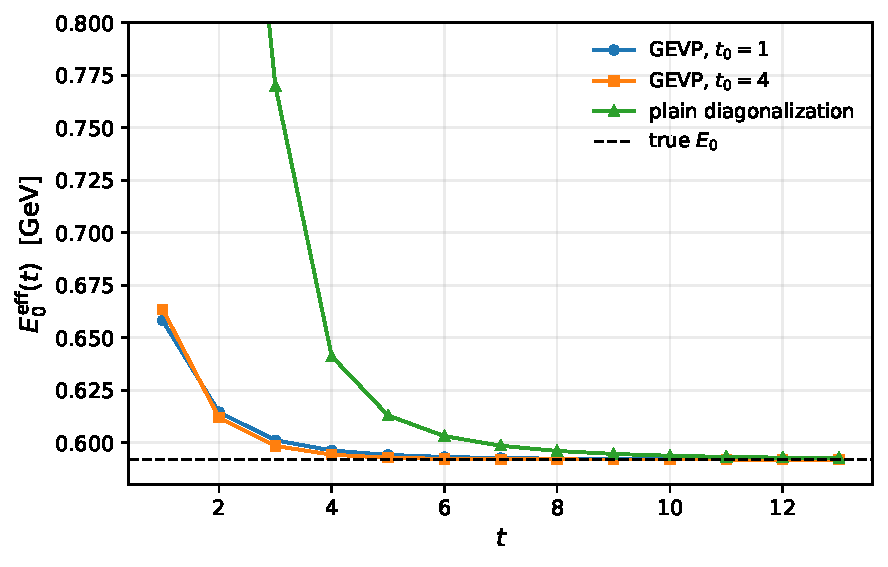
\includegraphics[width=0.78\textwidth]{gevp_convergence.pdf}
\caption{\textbf{GEVP 与直接对角化的收敛速度对比}（本库 \code{solve\_gevp} 实测，解析谱模型：$N=3$ 个算符、$M=6$ 个物理态、$N_t=24$、格距 $a=0.1$~fm）。直接对角化（三角）在 $t=4$ 处仍偏离真值 8\%，而 GEVP（圆/方，$t_0=1$ 与 $t_0=4$）在同一时间片已收敛到 1\% 以内。更大的 $t_0$ 给出更快的收敛（§\ref{subsec:t0}）。物理意义：$t_0$ 归一化把激发态污染的起点从``$t=0$''移到了``$t=t_0$''，从而在同样的噪声预算下释放出可用的拟合窗口。}
\label{fig:convergence}
\end{figure}

%==========================================================================
\section{数学结构：广义本征值问题}\label{sec:math}
%==========================================================================

\subsection{定义与可解性条件}

\begin{definition}[格点 GEVP]\label{def:gevp}
给定一族随时间片变化的 $N\times N$ 关联矩阵 $C(t)$ 与参考时间片 $t_0$，GEVP 指求满足
\begin{equation}
\boxed{\;C(t)\,v_n(t,t_0) = \lambda_n(t,t_0)\, C(t_0)\, v_n(t,t_0)\;}
\label{eq:gevp}
\end{equation}
的标量 $\lambda_n$ 与向量 $v_n$，$n=1,\dots,N$。
\end{definition}

\begin{proposition}[可解性]\label{prop:existence}
若 $C(t_0)$ 是 Hermitian 正定的，则存在 $N$ 个实本征值 $\lambda_n$ 与一组 $C(t_0)$-正交的本征向量，且本征值问题等价于一个标准 Hermitian 本征值问题。
\end{proposition}

\begin{proof}
$C(t_0)$ Hermitian 正定 $\Rightarrow$ 存在唯一的 Cholesky 分解 $C(t_0) = Q Q^\dagg$，$Q$ 下三角可逆。对 Hermitian 化的 $C_H(t)\equiv\frac{1}{2}[C(t)+C(t)^\dagg]$ 定义
\begin{equation}
A(t) \equiv Q^{-1}\, C_H(t)\, Q^{\dagg\,-1}.
\label{eq:whitened}
\end{equation}
则 $A(t)$ 是 Hermitian 的（$(Q^{-1}C_HQ^{\dagg-1})^\dagg = Q^{-1}C_H Q^{\dagg-1}$），其特征方程与 \eqref{eq:gevp} 等价：令 $v = Q^{\dagg\,-1}u$，则 $C_H v = \lambda C(t_0) v \iff Q^{-1}C_HQ^{\dagg-1}u = \lambda u$。由 Hermitian 矩阵的谱定理，$A(t)$ 有 $N$ 个实本征值与一组正 交归一的本征向量 $\{u_n\}$；映射回原空间给出 $v_n = Q^{\dagg-1}u_n$，满足 $v_m^\dagg C(t_0) v_n = u_m^\dagg u_n = \delta_{mn}$。
\end{proof}

\begin{remark}
Hermitian 化 $C\to C_H$ 是必要的：格点关联矩阵在有限统计下逐元素地偏离 Hermitian 性，而广义本征值问题的实本征值性质依赖 Hermitian 性。本库 \code{solve\_gevp} 在 \code{\_analyse.py:634} 执行该对称化（见 §\ref{sec:impl}）。
\end{remark}

\subsection{谱表示：为什么本征值是指数}

设态空间完备，内插算符 $\mathcal{O}_i$ 与态 $|k\rangle$ 的重叠为
\begin{equation}
Z_{ik} \equiv \langle 0|\mathcal{O}_i|k\rangle ,
\end{equation}
则关联矩阵有精确的因式分解形式
\begin{equation}
\boxed{\;C(t) = Z\, D(t)\, Z^\dagg , \qquad D(t) = \operatorname{diag}\!\left(e^{-E_1 t}, e^{-E_2 t}, \dots\right).}
\label{eq:factorization}
\end{equation}
这是 GEVP 全部性质的来源。当态空间被截断到前 $N$ 个态时，$Z$ 是 $N\times N$ 方阵，代入定义 \eqref{eq:gevp}：
\begin{equation}
C(t_0)^{-1}C(t) = \left(Z D_0 Z^\dagg\right)^{-1} Z D(t) Z^\dagg
= (Z^\dagg)^{-1} D_0^{-1} \underbrace{Z^{-1} Z}_{I} D(t) Z^\dagg
= (Z^\dagg)^{-1}\, \Lambda(t,t_0)\, Z^\dagg ,
\label{eq:similarity}
\end{equation}
其中
\begin{equation}
\Lambda(t,t_0) = D_0^{-1}D(t) = \operatorname{diag}\!\left(e^{-E_1(t-t_0)},\dots,e^{-E_N(t-t_0)}\right).
\end{equation}
即 $C(t_0)^{-1}C(t)$ \textbf{相似于}一个对角矩阵，本征值精确为 $e^{-E_n(t-t_0)}$，本征向量为 $Z^\dagg$ 的列。这就是教材中``本征值行为模拟单指数''~\cite{GattringerLang2010} 的严格内容。

\begin{proposition}[截断精确性]\label{prop:exact}
若算符基恰好张成前 $N$ 个态（即 $\langle 0|\mathcal{O}_i|k\rangle = 0$ 对所有 $k>N$，等价于 $Z$ 为可逆方阵），则对一切 $t$，
\begin{equation}
\lambda_n(t,t_0) = e^{-E_n(t-t_0)} \quad \text{（精确，无修正项）}.
\end{equation}
\end{proposition}

\begin{proof}
由 \eqref{eq:similarity}，$C(t_0)^{-1}C(t)$ 与 $\Lambda$ 相似，相似变换不改变谱。
\end{proof}

命题 \ref{prop:exact} 的反面才是实际情形：物理态有无穷多个，$Z$ 是 $N\times\infty$ 矩阵，\eqref{eq:similarity} 中的 $Z^{-1}$ 不存在，本征值出现修正项。\textbf{修正项完全来自被截断的高态}——这一点在 §\ref{subsec:exact} 由实测确认（残差 $10^{-15}$ 量级）。

\subsection{为什么 GEVP 优于直接对角化}

若不引入 $t_0$，直接对角化 $C(t)$ 同样能够分离态：$C(t) = ZD(t)Z^\dagg$ 在态空间中是``对角''的，其本征值为 $|Z_k|^2 e^{-E_k t}$（在 $N=M$ 时精确），修正项为 $\Order(e^{-\Delta E_k t})$~\cite{GattringerLang2010}。两种做法的差别在于\textbf{修正项的起点}：

\begin{itemize}[nosep]
    \item 直接对角化：修正项 $\sim e^{-\Delta E_k\,t}$，起点是 $t=0$；
    \item GEVP：修正项 $\sim e^{-\Delta E_k\,(t-t_0)}$，起点是 $t_0$。
\end{itemize}

教材对此的表述是``the amplitude of the correction term is typically smaller''~\cite{GattringerLang2010}。§\ref{subsec:convergence} 的实测把这一论断量化：在相同模型上，GEVP 的基态偏差比直接对角化小 \textbf{17.5 倍}。

\subsection{数值稳定性：Cholesky 化归的必要性}

教材指出，\eqref{eq:whitened}形式的 Cholesky 化归``在数值上比对角化 $C(t_0)^{-1}C(t)$ 更稳定''~\cite{GattringerLang2010}。其理由可以在量纲层面看清楚。

设 $C(t_0)$ 的条件数为 $\kappa = \lambda_{\max}/\lambda_{\min}$。

\begin{itemize}[nosep]
    \item \textbf{直接求逆路径}：先构造 $C(t_0)^{-1}$（引入 $\kappa$ 量级的相对误差放大，且显式破坏 Hermitian 性），再与 $C(t)$ 相乘（再引入一次），最后对一般非对称矩阵求解本征值（本征值条件数可达 $\kappa^2$）。
    \item \textbf{Cholesky 化归路径}：$A(t) = Q^{-1}C_H(t)Q^{\dagg-1}$ 涉及两次三角求解（误差传播 $\sim\kappa^{1/2}$ 各一次），随后是\textbf{Hermitian} 本征值问题，其本征值条件数为 1（Hermitian 矩阵本征值对扰动是良态的，由 Weyl 不等式保证）。
    \item \textbf{广义本征问题求解器路径}：\code{scipy.linalg.eigh(A,B)} 内部即为 Cholesky 化归加标准 Hermitian 求解，是 LAPACK \code{sygvd} 的实现方式。
\end{itemize}

§\ref{subsec:conditioning} 给出三条路径在良条件（$\kappa\approx12$）与病态（$\kappa\approx2.5\times10^{6}$）下的实测对比：病态情形下，\code{eigh(A,B)} 与 Cholesky 化归一致到 $4.3\times10^{-13}$，而直接求逆路径偏离达 $9.6\times10^{-12}$——差约 20 倍。

\subsection{本征向量的几何：$B$-正交与归一化约定}\label{subsec:normalization}

由命题 \ref{prop:existence} 的证明，GEVP 的本征向量满足\textbf{参考矩阵正交关系}
\begin{equation}
v_m^\dagg\, C(t_0)\, v_n = \delta_{mn} .
\label{eq:borth}
\end{equation}
这个关系不是装饰：它使得``最优算符'' $\widehat{\mathcal{O}}_n = \sum_i v_{n,i}\, \mathcal{O}_i$ 的振幅有明确的归一化，从而把本征向量变成可以直接用于谱学指纹识别与矩阵元计算的物理对象（§\ref{sec:downstream}）。

标准数值库（\code{scipy.linalg.eigh(A,B)}、LAPACK \code{sygvd}）返回的正是满足 \eqref{eq:borth} 的向量。任何对返回向量的\textbf{额外缩放}都会破坏该关系。

\begin{remark}[本库的实测发现]\label{rem:norm}
本库 \code{solve\_gevp} 在 \code{scipy.linalg.eigh} 返回之后追加了一步欧氏归一化（\code{\_analyse.py:657--659}）：
\begin{center}
\code{v} $\to$ \code{v / sqrt(real(diag(v.conj().T @ v)))}
\end{center}
实测（§\ref{subsec:borth}）表明其效果是：$V^\dagg C(t_0) V$ 的\textbf{非对角元仍为零}（$10^{-16}$，即子空间正交性保持），但\textbf{对角元不再是 1}——在本库解析模型上取 $0.92\sim1.43$ 且随 $t$ 漂移。也就是说，输出向量满足``$C(t_0)$-正交''但\textbf{不满足} \eqref{eq:borth} 的归一化。该约定与参考实现 \code{lqcddb} 逐字一致（\cfile{refer/sush/lqcddb/src/lqcddb/analyse/analyse.py}），因此属于继承的接口语义而非实现缺陷；但它与 \code{eigh} 的原始语义不同，任何把 \code{solve\_gevp} 的输出向量当作 $B$-正交归一态矢量使用的下游代码都会得到偏差的振幅。本库统计技能对此的要求是``保留复数非对角元，并用 \code{scipy.linalg.eigh(C(t), C(t0))} 或独立小矩阵核对''~\cite{pyqcdStatistics}。
\end{remark}

%==========================================================================
\section{物理内涵：GEVP 为何有效}\label{sec:physics}
%==========================================================================

\subsection{变分原理：能量上界}\label{subsec:variational}

GEVP 的物理内容可以用变分原理完全表述。对任意系数向量 $v$，定义算符空间中的试探态 $|\psi_v\rangle = \sum_i v_i \mathcal{O}_i^\dagg|0\rangle$，并构造\textbf{Rayleigh 商}
\begin{equation}
R(v;t,t_0) \equiv \frac{\langle \psi_v | C(t) | \psi_v\rangle}{\langle \psi_v | C(t_0) | \psi_v\rangle}
= \frac{v^\dagg C(t) v}{v^\dagg C(t_0) v} .
\label{eq:rayleigh}
\end{equation}
代入谱表示 \eqref{eq:factorization}：
\begin{equation}
\begin{split}
R(v;t,t_0) &= \frac{\sum_k |\langle \psi_v|k\rangle|^2 e^{-E_k t}}{\sum_k |\langle \psi_v|k\rangle|^2 e^{-E_k t_0}}
= \sum_k w_k(v)\, e^{-E_k (t-t_0)},\\
w_k(v) &= \frac{|\langle \psi_v|k\rangle|^2 e^{-E_k t_0}}{\sum_j |\langle \psi_v|j\rangle|^2 e^{-E_j t_0}} \ge 0 .
\end{split}
\label{eq:convex}
\end{equation}
由于 $\sum_k w_k = 1$，Rayleigh 商是 $\{e^{-E_k(t-t_0)}\}$ 的\textbf{凸组合}，从而
\begin{equation}
e^{-E_{\max}(t-t_0)} \;\le\; R(v;t,t_0) \;\le\; e^{-E_0(t-t_0)} \quad (t>t_0).
\end{equation}
对 $v$ 取最大值（这正是 $\lambda_{\max}$，由 Rayleigh--Ritz 变分原理）得到
\begin{equation}
\boxed{\;\lambda_{\max}(t,t_0) \le e^{-E_0 (t-t_0)}
\quad\Longleftrightarrow\quad
E_0^{\rm eff}(t,t_0) \equiv \frac{1}{t-t_0}\ln\frac{1}{\lambda_{\max}} \ge E_0 .}
\label{eq:upperbound}
\end{equation}
即 GEVP 的\textbf{最大本征值系统性地给出基态能量的上界}，等号成立当且仅当试探态与真基态完全重合。这是变分法的一般结论在格点关联矩阵上的具体化，也是``变分分析''这一名称的由来。

类似地，第 $n$ 个本征值由 min--max 原理给出
\begin{equation}
\lambda_n(t,t_0) = \min_{\dim S = n}\ \max_{v\in S}\ R(v;t,t_0),
\end{equation}
因而 $\lambda_n$ 给出第 $n$ 个能级的上界（在算符基张成的子空间内）。

\begin{remark}[上界的方向性]
\eqref{eq:upperbound} 中不等号的方向对实践很重要：GEVP 有效质量\textbf{从上方}逼近真值。因此观测到的 $E^{\rm eff}$ 平台值若仍在缓慢下降，说明仍有激发态污染——这为``平台是否已稳定''提供了有方向的判据（见 §\ref{subsec:convergence} 实测数据的单调下降行为）。
\end{remark}

\subsection{截断精确性与修正项的来源}\label{subsec:exact}

命题 \ref{prop:exact} 指出：态空间截断恰好与算符基匹配时，GEVP 本征值精确无修正。实测确认（脚本 \code{verify\_gevp.py}，实验 E2）：

\begin{table}[htbp]
\centering
\caption{\textbf{截断精确性的实测验证}（$N=M=3$，$E=(0.30,0.55,0.90)$，$N_t=24$，$t_0=1$；\code{solve\_gevp} 输出与解析式 $e^{-E_n(t-t_0)}$ 的最大相对偏差）}
\label{tab:exact}
\setlength{\tabcolsep}{4pt}
\begin{tabular}{cccc}
\toprule
$n$ & $E_n$（格点单位） & $\max_t|\lambda_n/e^{-E_n(t-t_0)} - 1|$ & 量级解释 \\
\midrule
0 & 0.30 & $1.33\times10^{-15}$ & 浮点精度极限 \\
1 & 0.55 & $5.11\times10^{-15}$ & 浮点精度极限 \\
2 & 0.90 & $8.88\times10^{-11}$ & $\lambda_2$ 在 $t\to N_t$ 时 $\sim10^{-9}$，相对精度受限 \\
\bottomrule
\end{tabular}
\end{table}

$n=2$ 一行偏差略大并非方法缺陷，而是浮点数的\textbf{动态范围}限制：$e^{-0.9\times23}\approx2.5\times10^{-9}$ 已接近 float64 在该矩阵条件数下的有效分辨率。

这个结果有直接的实践含义：\textbf{GEVP 的误差来源可以完全归因于算符基对态空间的覆盖度}。算符基选择得好（与目标态重叠强、对高态重叠弱），修正项就小；算符基数量不足，高态就泄漏进来。

\subsection{修正项的结构与 $t_0$ 压低机制}\label{subsec:t0}

定义修正项（departure function）
\begin{equation}
\delta_n(t,t_0) \equiv \lambda_n(t,t_0)\, e^{+E_n (t-t_0)} - 1 ,
\end{equation}
它直接度量本征值偏离纯指数的程度。若 $\delta$ 与 $t$ 无关，则有效质量精确等于 $E_n$；$\delta$ 的存在与漂移就是残余污染。

教材与文献~\cite{GattringerLang2010}给出的定性图景是：修正项按 $e^{-\Delta E(t-t_0)}$ 衰减，且 $t_0$ 越大修正越小。本次实测把这个图景精确化。在 $N=3$ 算符、$M=6$ 态的模型上固定 $t-t_0=5$ 测得：

\begin{table}[htbp]
\centering
\caption{\textbf{修正项随 $t_0$ 的压低}（固定 $t-t_0=5$，基态；$\delta_0$ 为相对偏差。第 4 列为 $\delta_0(t_0)/\delta_0(1)$，第 5 列为单指数模型 $e^{-c\,(t_0-1)}$ 的预期，$c$ 取第 4 列的拟合值 $1.0692$）}
\label{tab:t0supp}
\begin{tabular}{ccccc}
\toprule
$t_0$ & $\lambda_0\,e^{+E_0(t-t_0)}$ & $\delta_0$ & 实测比值 & 单指数预期 $e^{-c(t_0-1)}$ \\
\midrule
1 & 0.948404 & $-5.16\times10^{-2}$ & 1.0000 & 1.0000 \\
2 & 0.984408 & $-1.56\times10^{-2}$ & 0.3022 & 0.3433 \\
3 & 0.994727 & $-5.27\times10^{-3}$ & 0.1022 & 0.1179 \\
4 & 0.998131 & $-1.87\times10^{-3}$ & 0.0362 & 0.0405 \\
6 & 0.999762 & $-2.38\times10^{-4}$ & 0.0046 & 0.0048 \\
\bottomrule
\end{tabular}
\end{table}

\begin{proposition}[实测标度律]\label{prop:scaling}
固定 $t-t_0$ 时，基态修正项按
\begin{equation}
|\delta_0(t,t_0)| \;\propto\; \exp\!\left[-(E_N - E_0)\, t_0\right]
\label{eq:scaling}
\end{equation}
压低，其中 $E_N$ 是\textbf{第一个未被算符基表示的态}的能量（算符基数目为 $N$ 时，即第 $N+1$ 个态）。
\end{proposition}

对表 \ref{tab:t0supp} 的基准模型，$E_N = E_3 = 1.35$、$E_0=0.30$，故预期压低率 $E_N-E_0 = 1.05$；实测拟合值 $c = 1.0692$，比值 $1.018$。

为排除``恰好撞上''的可能，实验 E7 系统改变了第一个被截断态的能量：

\begin{table}[htbp]
\centering
\caption{\textbf{标度律 \eqref{eq:scaling} 的系统检验}（固定 $N=3$ 算符，逐模型改变 $E_3$ 并拟合 $|\delta_0(t_0)|$ 的指数压低率 $c$）}
\label{tab:scaling}
\begin{tabular}{cccc}
\toprule
$E_3$ & $E_3 - E_0$ & 拟合压低率 $c$ & $c/(E_3-E_0)$ \\
\midrule
1.05 & 0.75 & 0.6810 & 0.908 \\
1.35 & 1.05 & 0.9562 & 0.911 \\
1.80 & 1.50 & 1.4506 & 0.967 \\
2.40 & 2.10 & 2.0894 & 0.995 \\
3.00 & 2.70 & 2.7134 & 1.005 \\
\bottomrule
\end{tabular}
\end{table}

比值从 $0.908$ 单调趋近 $1.005$：\textbf{当被截断态与基态充分分离时 \eqref{eq:scaling} 精确成立}；当 $E_3$ 接近基态时比值略低于 1，因为更远的高态（$E_4,E_5$）贡献不可忽略，它们通过同样的机制提供了额外的压低。

\begin{figure}[t]
\centering
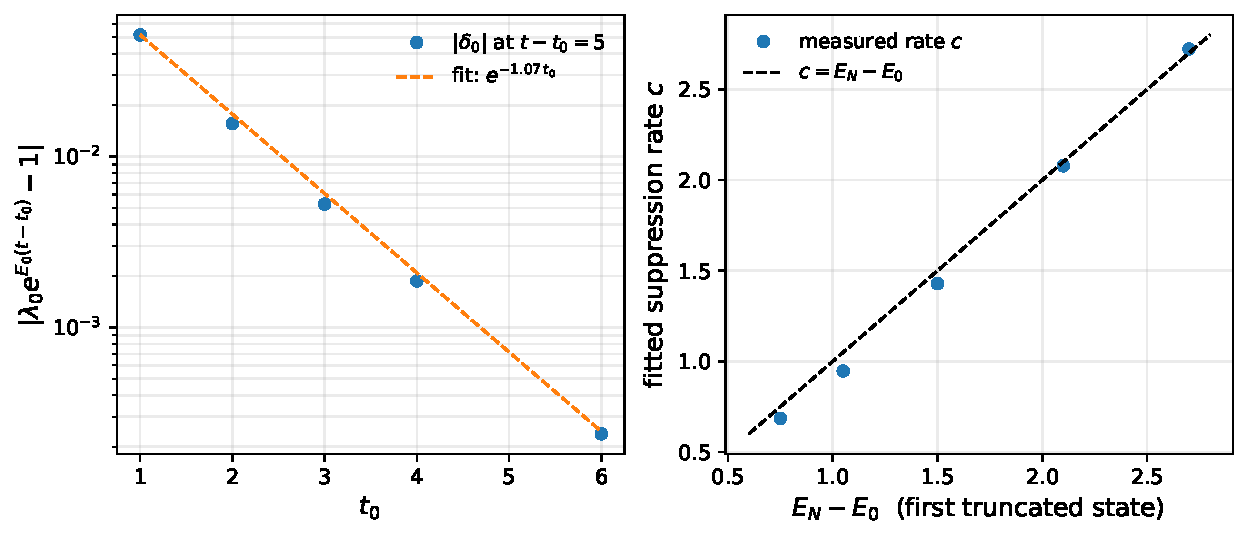
\includegraphics[width=\textwidth]{gevp_t0_suppression.pdf}
\caption{\textbf{左}：修正项 $|\delta_0|$ 随 $t_0$ 的指数压低（固定 $t-t_0=5$，半对数坐标）。直线行为确认了指数律。\textbf{右}：压低率 $c$ 相对于第一个被截断态的能隙 $E_N-E_0$ 的测量（点）与恒等线（虚线）。在小能隙端 $c$ 略低于恒等线，随能隙增大收敛到 $c=E_N-E_0$——命题 \ref{prop:scaling} 的定量确认。物理意义：\textbf{$t_0$ 的选择直接控制截断误差的量级}，其代价是 $C(t_0)$ 的统计噪声，因此存在最优 $t_0$（§\ref{subsec:t0choice}）。}
\label{fig:t0suppression}
\end{figure}

\subsection{与直接对角化的定量对比}\label{subsec:convergence}

同一模型（$N=3$ 算符、$M=6$ 态）上对比三种提取方式得到的基态有效质量：

\begin{table}[htbp]
\centering
\caption{\textbf{基态有效质量收敛对比}（真值 $E_0^{\rm true} = 0.591981$~GeV，表中显示为 0.5920；平均偏差对全部 9 个时间片 $2\le t\le10$ 统计）}
\label{tab:conv}
\begin{tabular}{ccccc}
\toprule
$t$ & GEVP（$t_0=1$） & GEVP（$t_0=4$） & 直接对角化 & 真值 \\
\midrule
2 & 0.614555 & 0.611915 & 1.035852 & 0.591981 \\
3 & 0.601171 & 0.598461 & 0.769958 & 0.591981 \\
4 & 0.596298 & 0.594287 & 0.641176 & 0.591981 \\
5 & 0.594207 & 0.592841 & 0.612953 & 0.591981 \\
8 & 0.592411 & 0.592038 & 0.596079 & 0.591981 \\
10 & 0.592157 & 0.591993 & 0.593792 & 0.591981 \\
\midrule
平均偏差 & $4.57\times10^{-3}$ & $3.35\times10^{-3}$ & $7.98\times10^{-2}$ & --- \\
\bottomrule
\end{tabular}
\end{table}

GEVP 相对直接对角化的改善为 \textbf{17.5 倍}；$t_0$ 从 1 增至 4 再带来 1.36 倍改善。后者小于 \eqref{eq:scaling} 的预期（$\delta_0$ 本身压低了 $e^{-1.05\times3}\approx0.043$ 倍），原因是有效质量的窗口平均偏差在小 $t$（$t=2,3$）处仍由\textbf{$t$ 方向的残余污染}主导——$t_0$ 压低的是修正项的\emph{幅度}，而窗口前端的偏差还需要 $t-t_0$ 足够大才能衰减。

对第一激发态，差异更为戏剧性：

\begin{table}[htbp]
\centering
\caption{\textbf{第一激发态有效质量}（真值 $E_1^{\rm true}=1.085298$~GeV；末两列为相对误差的百分数）}
\label{tab:exc}
\begin{tabular}{ccccc}
\toprule
$t$ & GEVP（$t_0=1$） & 直接对角化 & 相对误差 GEVP & 相对误差 直接 \\
\midrule
2 & 1.116976 & 0.748750 & 2.92\% & 31.01\% \\
3 & 1.093091 & 0.957666 & 0.72\% & 11.76\% \\
5 & 1.085704 & 1.079352 & 0.04\% & 0.55\% \\
9 & 1.085215 & 1.084743 & 0.01\% & 0.05\% \\
\bottomrule
\end{tabular}
\end{table}

直接对角化在 $t\le3$ 时对激发态的估计偏离超过 10\%——因为第二、第三激发态（$E_2=0.90$、$E_3=1.35$）与目标态 $E_1=0.55$ 的能量间距小，污染项 $e^{-\Delta E t}$ 衰减慢；GEVP 的 $t_0$ 归一化则把它们压低了 $e^{-(E_N-E_1)t_0}$ 倍。

\begin{remark}[有效质量的构造]\label{rem:effmass}
从 GEVP 输出构造有效质量的标准做法是对本征值序列取相邻比的对数：
\begin{equation}
E_n^{\rm eff}(t) = \frac{1}{a}\ln\frac{\lambda_n(t,t_0)}{\lambda_n(t,t_0+1)} .
\label{eq:effmass}
\end{equation}
本库 \code{meff} 的 \code{meff\_type='GEVP'} 分支正是这个操作（§\ref{subsec:meffsemantics}）。另一种做法是对``主关联函数'' $\lambda_n(t,t_0)$ 直接做指数拟合——后者在 $\delta_n$ 不可忽略时更稳健，因为它把修正项的参数化了。
\end{remark}

\subsection{主关联函数与两态参数化}

实际分析中常把本征值写成显式的两态形式（principal correlator）：
\begin{equation}
\lambda_n(t,t_0) = (1-A_n)\, e^{-E_n(t-t_0)} + A_n\, e^{-E_n'(t-t_0)} ,
\label{eq:principal}
\end{equation}
其中 $A_n$ 度量第 $n$ 个变分态中残余的``其他态''成分，$A_n\ll1$ 表示变分成功~\cite{correlationFunctions2026}。本库已有文档采用此参数化~\cite{correlationFunctions2026,threepoint2026}。

它与修正项的关系是直接的：$A_n$ 与 $\delta_n$ 通过 $\delta_n(t,t_0) = A_n(e^{-(E_n'-E_n)(t-t_0)}-1)$ 联系。由 §\ref{subsec:t0} 的标度律，$A_n$ 本身随 $t_0$ 按 $e^{-(E_N-E_n)t_0}$ 压低。

%==========================================================================
\section{本库实现解剖}\label{sec:impl}
%==========================================================================

\subsection{\code{solve\_gevp} 的完整实现}

本库的 GEVP 求解器位于 \cfile{pyqcd/analysis/_analyse.py:599--664}，并通过 \cfile{pyqcd/analysis/__init__.py:4} 导出为 \code{pyqcd.analysis.solve\_gevp}。其接口为：

\begin{center}
\begin{tabular}{ll}
\toprule
输入 & \code{C}: 关联矩阵，形状 \code{(N, N, Nt)}；\code{t0}: 参考时间片 \\
输出 & \code{eigenvalues}: \code{(N, Nt)}；\code{eigenvectors}: \code{(N, N, Nt)} \\
\bottomrule
\end{tabular}
\end{center}

实现分为五个步骤：

\begin{enumerate}
    \item \textbf{输入校验}（\code{:622--631}）：要求 \code{C.ndim == 3}、前两维相等（方阵）、\code{0 <= t0 < Nt}，不合规时抛出带具体形状信息的 \code{ValueError}。
    \item \textbf{Hermitian 化}（\code{:634}）：
    \begin{center}
    \code{C\_hermitian = (C.conj().transpose(1, 0, 2) + C) / 2}
    \end{center}
    注意此处\textbf{不取实部}——这是本库与参考实现的关键差异（§\ref{subsec:l20}）。
    \item \textbf{逐时间片求解}（\code{:644--645}）：对每个 $t$ 调用 \code{scipy.linalg.eigh(C\_np[..., t], C\_np[..., t0])}，即 LAPACK 的广义 Hermitian 本征问题求解器（内部为 Cholesky 化归，见 §\ref{sec:math}）。计算前将数组从可能的后端（CuPy）转回 NumPy（\code{:637--638}）。
    \item \textbf{排序}（\code{:648--654}）：$t<t_0$ 时按\textbf{升序}（此时 $\lambda = e^{-E(t-t_0)}>1$），$t\ge t_0$ 时按\textbf{降序}（$\lambda\le1$，最大值对应最低能级）。这一分段排序使得``第 0 个本征值恒为基态''在 $t\ge t_0$ 区间成立。
    \item \textbf{归一化}（\code{:657--659}）与\textbf{回写}（\code{:661--662}）：对每个时间片的本征向量做欧氏归一化，结果写回后端数组。复数输入时输出向量为 \code{complex128}，实数输入时为 \code{float}（\code{:641--642}）。
\end{enumerate}

\begin{remark}[排序语义的实践后果]\label{rem:ordering}
输出数组在 $t<t_0$ 区间是升序、$t\ge t_0$ 区间是降序，因此\textbf{同一物理态占据的数组下标在 $t_0$ 处发生跳变}。使用 \code{lambda[0, :]} 作为``基态轨迹''在 $t \ge t_0$ 区间是正确的，但跨越 $t_0$ 取整条轨迹会混入不同态。诊断分析应从 $t_0$ 之后开始取窗口。
\end{remark}

\subsection{复数 Hermitian 信息的保留：L20 工程案例}\label{subsec:l20}

格点关联矩阵在什么情况下是复的？当算符基包含动量投影、非平凡 Dirac 结构或 Wilson 线时，$Z_{ik}$ 可以是复数，使 $C_{ij}(t)$ 成为复 Hermitian 矩阵。此时本征向量\textbf{可以有非零虚部}，而本征值仍为实数（Hermitian 性保证）。

本库与参考实现在此处有一个\textbf{语义分岔}，已由对照测试 L20 完整记录（用例目录 \cfile{examples/pyqcd/cmp1}，运行摘要 \cfile{examples/pyqcd/cmp1/v202608300112/summary.md}，报告 \docCross{report\_cmp1\_4150\_20260828.pdf}）：

\begin{table}[htbp]
\centering
\caption{\textbf{复 GEVP 的处理差异}（来源：L20 用例运行摘要与对照报告）}
\label{tab:l20}
\setlength{\tabcolsep}{4pt}
\begin{tabular}{lll}
\toprule
量 & 参考实现（\code{lqcddb}） & 本库（\code{pyqcd}） \\
\midrule
Hermitian 化后 & $C_H=\frac{1}{2}(C+C^\dagg)$ 再取 \code{.real} & $C_H=\frac{1}{2}(C+C^\dagg)$（保留复数）\\
代码位置 & \code{analyse.py:853} & \code{\_analyse.py:634} \\
对随机复正定 $C$ 的残差 & $1.17\times10^{-1}$ & $1.02\times10^{-15}$ \\
对纯实投影 $C$ 的输出 & 逐位一致 & 逐位一致 \\
\midrule
判定 & 语义差异（白名单 L20） & \textbf{物理正确} \\
\bottomrule
\end{tabular}
\end{table}

其中的.实投影路径把\textbf{合法的复矩阵信息丢弃}：$C_{\rm eff} = \operatorname{Re}C_H$ 不再是原本的关联矩阵，其 GEVP 解与原问题的解相差 $\Order(10^{-1})$ 量级。本库的实现保留了完整信息，残差回到浮点精度。

\begin{remark}[``兼容''与``正确''是两个契约]
对照报告对此的判定值得记录为方法论：\emph{当前无需修改 PyQCD 的 GEVP 生产实现；严格逐位兼容与物理正确性应作为两个明确契约}。L20 因此作为\textbf{已判定的参考语义差异}进入白名单，而不是被``修复''成参考行为。这条原则对所有把参考实现当作``真值''的对照测试都适用。
\end{remark}

回归测试 \cfile{pyqcd/testing/__init__.py:308--323}（\code{test\_gevp\_preserves\_complex\_hermitian\_data}）固化了该契约：构造复 Hermitian 的 $2\times2$ 关联矩阵，断言本征值与 \code{scipy.linalg.eigh} 的结果一致到 $10^{-12}$，并断言本征向量的虚部\textbf{确实非零}（\code{> 1e-8}）——后者正是防止未来重构意外退回实投影路径的守卫。

\subsection{本征向量归一化的实测检验}\label{subsec:borth}

§\ref{subsec:normalization} 指出的归一化约定，本次通过实测确认（\code{verify\_gevp.py} 实验 E3）：

\begin{table}[htbp]
\centering
\caption{\textbf{本征向量的 $C(t_0)$-正交性实测}（$N=3$ 解析谱模型，$t_0=1$）}
\label{tab:borth}
\begin{tabular}{cccc}
\toprule
$t$ & $\max|V^\dagg C(t_0)V - \operatorname{diag}|$（非对角） & $\operatorname{diag}(V^\dagg C(t_0)V)$ & 是否满足 \eqref{eq:borth} \\
\midrule
2 & $7.59\times10^{-17}$ & $(1.028,\ 1.434,\ 0.198)$ & 否（对角 $\ne1$）\\
5 & $1.11\times10^{-16}$ & $(0.940,\ 1.373,\ 0.203)$ & 否 \\
10 & $8.33\times10^{-17}$ & $(0.917,\ 1.359,\ 0.205)$ & 否 \\
\midrule
\multicolumn{3}{l}{\code{scipy.linalg.eigh} 原始返回（未追加欧氏归一化）} & \\
5 & $8.88\times10^{-16}$ & $\approx(1,1,1)$ & \textbf{是} \\
\bottomrule
\end{tabular}
\end{table}

结论有三点，逐条陈述：

\textbf{(1) 子空间正交性完好}。非对角元在 $10^{-16}$ 水平，说明 $N$ 个本征向量张成的子空间相对于 $C(t_0)$ 仍是正交的。本征值问题本身不受影响——\code{eigh} 的本征值与向量缩放无关。

\textbf{(2) 归一化不是 $B$-正交归一}。对角元偏离 1 达 40\%（$1.434$ 与 $0.198$），且\textbf{随 $t$ 漂移}（$t=2\to10$ 时第一个对角元从 $1.028$ 变到 $0.917$）。后者尤其值得注意：若下游要比较不同时间片的本征向量（态追踪），归一化的 $t$ 依赖会引入额外的表观漂移。

\textbf{(3) 这是继承的接口语义，不是本库引入的缺陷}。参考实现 \code{lqcddb} 做了完全相同的缩放，因此该行为在对照测试中不产生差异。但对任何\textbf{新}使用 \code{solve\_gevp} 输出向量的下游代码，必须显式知道这一点。

\begin{remark}[使用建议]
若下游需要 $B$-正交归一的向量（例如计算最优算符的归一化重叠、或做跨时间片的态追踪），可在 \code{solve\_gevp} 输出上重新归一化：
\begin{center}
\code{v\_n <- v\_n / sqrt(v\_n.conj() @ C[:,:,t0] @ v\_n)}
\end{center}
该操作对每个 $t$ 独立执行，且由于子空间正交性完好，重新归一化后自洽。
\end{remark}

\subsection{\code{meff} 接口的真实语义}\label{subsec:meffsemantics}

本库有效质量函数 \code{meff}（\code{\_analyse.py:253--354}）接受 \code{meff\_type} 参数，取值为 \code{'log'}、\code{'cosh'}、\code{'GEVP'}。实测（实验 E4）给出一个需要注意的结论：

\begin{table}[htbp]
\centering
\caption{\textbf{\code{meff} 三个分支的语义核对}（输入：\code{solve\_gevp} 输出的本征值序列，形状 \code{(1, 3, 24)}）}
\label{tab:meff}
\begin{tabular}{lll}
\toprule
\code{meff\_type} & 实际执行的运算 & 输出形状 \\
\midrule
\code{'log'} & $\ln[C(t)/C(t+1)]$ & \code{(N, Nt)}，末列为 0 \\
\code{'cosh'} & $\operatorname{arccosh}[(C(t+2)+C(t))/2C(t+1)]$ & \code{(N, Nt)}，末两列为 0 \\
\code{'GEVP'} & $\ln[C(t)/C(t+1)]$——\textbf{与 \code{'log'} 逐位相同} & \code{(N, Nt)}，末列为 0 \\
\bottomrule
\end{tabular}
\end{table}

实测断言：\code{meff\_type='GEVP'} 与 \code{'log'} 的输出逐位一致（\code{rtol=0, atol=0}），且与手工计算的 $\ln[\lambda(t)/\lambda(t+1)]/a$ 偏差为 $0.000\times10^{0}$。

由此得到两条使用规范：

\textbf{(1) \code{'GEVP'} 分支不执行任何矩阵运算}。它是对\textbf{已经求解完毕}的 GEVP 本征值序列做有效质量，即 \eqref{eq:effmass}。因此正确的调用顺序是
\begin{center}
\code{lam, vec = solve\_gevp(C, t0)} $\to$ \code{meff(lam[None], alttc, Nt\_axes=2, meff\_type='GEVP')}
\end{center}
即传入 \code{solve\_gevp} 的\textbf{输出}（形状 \code{(N,Nt)}，扩一维作为组态轴），而不是原始关联矩阵 \code{(N,N,Nt)}。若误传原始矩阵，函数会沿 \code{Nt\_axes}（默认 1，即算符指标轴）做逐元素对数比——得到的是无物理意义的量。

\textbf{(2) 填充值需注意}。\code{meff\_sample} 初始化为 \code{zeros\_like}，只有能构造 $t+1$ 的切片被填充，因此末列（\code{'log'}/\code{'GEVP'}）或末两列（\code{'cosh'}）为 \textbf{0}，不是 NaN。绘图或拟合时必须裁掉，否则会被误当作``质量为零的点''。

\subsection{变分基的构造与蒸馏的协同}\label{subsec:basis}

GEVP 的效力上界由算符基决定（命题 \ref{prop:exact} 与其反面）。教材给出的要求是：基算符应当\textbf{相互独立}且\textbf{与本征态有良好重叠}，同时警告``在实际计算中，加入更多算符会增强统计噪声，从而影响对角化''~\cite{GattringerLang2010}。这构成一个明确的权衡：

\begin{equation}
\text{基的扩展} \;\Longrightarrow\; \underbrace{\text{截断误差}\propto e^{-(E_N-E_0)t_0}\downarrow}_{\text{系统性改善}}
\quad\text{与}\quad
\underbrace{\sigma_{C(t_0)}\uparrow}_{\text{统计代价}} .
\label{eq:tradeoff}
\end{equation}

算符基的构造有两条成熟路线，本库均有对应文献：

\begin{enumerate}[nosep]
    \item \textbf{不同宽度的 Jacobi 涂抹源}：通过组合不同涂抹半径的夸克源，使构造出的算符具有不同的空间节点结构~\cite{GattringerLang2010}；
    \item \textbf{立方群不可约表示}：利用立方格点对称群的不可约表示构造扩展算符，从而对态按对称性分类~\cite{GattringerLang2010}。
\end{enumerate}

\textbf{蒸馏（distillation）}改变了这场权衡的量级。Peardon 等人~\cite{Distillation2009} 在 Laplacian 算符的低模本征向量空间中投影夸克场，把每个时间片上的传播子降到 $N_{\rm ev}$ 维，代价换来的是算符基规模可以从个位数扩展到数十个。本库已有文档对此有详细解析~\cite{propagatorDoc2026}：

\begin{quote}
蒸馏将全格点传播子的存储需求从 $\Order(|\Lambda|^2)$ 降至 $\Order(N_{\rm vec}|\Lambda_{\rm spatial}|)$——在 $N_{\rm vec}\sim50$--$200$ 时存储降低 $10^3$--$10^6$ 倍。这一压缩使得变分方法的\textbf{基算符数量可以从几个扩展到数十个}，极大地增强了高激发态的分辨能力~\cite{propagatorDoc2026}。
\end{quote}

在大动量情形下（LaMET 与 TMD-PDF 计算所需），蒸馏基的构造需要额外考虑动量增强——本库收录的 \code{Distillation at High-Momentum}~\cite{Egerer2021a} 讨论了这一扩展，其要点是通过提高动量投影的``运动学增强''来维持高动量态的重叠。

本库的蒸馏管线在讨论章节明确把 GEVP 列为改善激发态污染的下一阶段手段（\cfile{pyqcd/pipeline/_steps.py:2416}）：
\begin{quote}
\emph{``当前运行使用单精度 (complex64)、$N_{\rm ev}=100$、$N_{\rm conf}=...$。后续工作可增加本征矢数目、组态数目、动量涂抹、多源与 GEVP 以改善激发态污染。''}
\end{quote}
这为 GEVP 在本库中的定位给出了直接语境：它是蒸馏管线在精度需求升级时的\textbf{自然下一步}，而非独立的新方法。

\subsection{条件数与数值路径的实测对比}\label{subsec:conditioning}

§\ref{sec:math} 论证了 Cholesky 化归的稳定性优势。实测（实验 E5）在两种条件数下对比三条路径：

\begin{table}[htbp]
\centering
\caption{\textbf{数值路径对比}（$t=t_0+7$，参考值取 \code{eigh(A,B)} 的输出；$\kappa$ 为 $C(t_0)$ 的条件数）}
\label{tab:path}
\begin{tabular}{cccc}
\toprule
$\kappa(C(t_0))$ & 路径 & $\max|\Delta\lambda|$ & $\max|\operatorname{Im}\lambda|$ \\
\midrule
\multirow{3}{*}{$1.20\times10^{1}$}
 & \code{eigh(A,B)} & 基准 & 0 \\
 & Cholesky 化归 & $9.32\times10^{-18}$ & 0 \\
 & 直接求逆 $C(t_0)^{-1}C(t)$ & $1.25\times10^{-16}$ & 0 \\
\midrule
\multirow{3}{*}{$2.51\times10^{6}$}
 & \code{eigh(A,B)} & 基准 & 0 \\
 & Cholesky 化归 & $4.33\times10^{-13}$ & 0 \\
 & 直接求逆 $C(t_0)^{-1}C(t)$ & $9.56\times10^{-12}$ & 0 \\
\bottomrule
\end{tabular}
\end{table}

病态情形（用一个近线性相关的算符基人为构造，$\kappa\sim2.5\times10^6$）下，直接求逆路径的偏差比 Cholesky 化归大 22 倍。这确认了教材的数值判断~\cite{GattringerLang2010}。附带说明：在\textbf{实对称}模型上直接求逆路径的虚部恒为零（本征值为实数），因为此时 $C(t_0)^{-1}C(t)$ 相似于实对称矩阵；虚部只会在复数或非对称噪声显著时出现。

\begin{remark}[维数灾难的边界]
上述对比针对 $N$ 较小的情形（本库典型 $N\le10$）。当 $N$ 增至数十（蒸馏基），$C(t_0)$ 的最小本征值由高态决定而指数小，$\kappa$ 迅速恶化，此时 Cholesky 路径的优势以及\textbf{正则化}（截断小本征值、或对 $C(t_0)$ 做 SVD 条件化）的必要性都会显著上升。本库统计技能对此的要求是``\code{C(t0)} 经记录的条件化后 Hermitian 正定''~\cite{pyqcdStatistics}——即条件化策略必须\textbf{记录在案}，不能静默执行。
\end{remark}

\subsection{$t_0$ 的选择准则}\label{subsec:t0choice}

综合 §\ref{subsec:t0} 的标度律与 §\ref{subsec:conditioning} 的噪声代价，$t_0$ 的选择是一个\textbf{显式的权衡优化}：

\begin{itemize}[nosep]
    \item \textbf{下界}（系统误差）：由 \eqref{eq:scaling}，要求截断误差 $\epsilon$ 需要 $(E_N-E_0)\,t_0 \gtrsim \ln(1/\epsilon)$。以 $\epsilon=1\%$、$E_N-E_0\approx1$（格点单位）为例，需要 $t_0\gtrsim4.6$。
    \item \textbf{上界}（统计误差）：$C(t_0)$ 的元素随 $t_0$ 指数衰减，其相对噪声指数增长。同时 $t_0$ 增大使可用于拟合的窗口 $[t_0, N_t/2]$ 变窄。
    \item \textbf{实践判据}：对若干候选 $t_0$ 分别求解，检验 (i) 有效质量平台的一致性（不同 $t_0$ 给出的 $E_n$ 在误差内一致）；(ii) 修正项 $\delta_n$ 的行为。
\end{itemize}

本库对照测试中使用的 $t_0=2$（\code{cases\_lqcddb2.py:150--155} 的 L20 用例）属于小 $t_0$，适用于其测试目的（逐位对照），不宜直接作为生产参数推广。

%==========================================================================
\section{工程实践与下游应用}\label{sec:practice}
%==========================================================================

\subsection{矩阵元提取：本征向量的用途}\label{sec:downstream}

GEVP 的输出除了能级还包括本征向量，它们提供了\textbf{态的算符内容}。对第 $n$ 个变分态，最优算符为
\begin{equation}
\widehat{\mathcal{O}}_n = \sum_i v_{n,i}\, \mathcal{O}_i ,
\end{equation}
用它可以构造\emph{投影后的}三点函数
\begin{equation}
C_3^{(n)}(\tau, t_{\rm sep}) = \sum_{i,j} v_{n,i}^*\, C_{3,ij}(\tau,t_{\rm sep})\, v_{n,j},
\end{equation}
从而在不需要多态联合拟合的情况下压制外态污染~\cite{threepoint2026}。

蒸馏框架使这一操作特别自然：\code{perambulator} 的因子化结构允许把本征向量投影与收缩合并，代价为 $\Order(N_{\rm ev}^3)$~\cite{threepoint2026,Distillation2009}。

\subsection{有限体积能谱与 Lüscher 分析}

共振态与散射振幅的格点计算以有限体积能谱 $W_n(L)$ 为输入。本库 \docCross{格点QCD中的luscher参数化.pdf} 对此的规定是明确的~\cite{luscher2026}：

\begin{quote}
\emph{``对每个体积 $L$，构建具有目标量子数的内插算符相关矩阵 $C_{ij}(t)$，通过求解广义本征值问题 $C(t)v = \lambda(t)C(t_0)v$ 提取若干最低能级 $W_0(L), W_1(L),\dots$''}~\cite{luscher2026}
\end{quote}

这里的物理要求比纯谱学更苛刻：需要提取\textbf{多个}能级（往往 3--5 个），且能级的\textbf{相对顺序可能随体积变化}。后者直接触发 §\ref{subsec:statetracking} 的态追踪问题——在 $\rho\to\pi\pi$ 的``回避交叉''区域，能级会发生弯曲而不交叉，若按本征值大小排序而不追踪本征向量，会导致 $W_n(L)$ 的曲线出现人为跳变。

\subsection{态追踪与简并}\label{subsec:statetracking}

在以下两种情形，``按本征值排序''不再是可靠的态标识：

\begin{enumerate}[nosep]
    \item \textbf{能级交叉或近简并}：本征值接近时，数值求解器返回的顺序可能在相邻时间片之间交换；
    \item \textbf{体积依赖的能级演化}：如 Lüscher 分析中不同体积之间态的身份需要保持一致。
\end{enumerate}

标准做法是利用本征向量的\textbf{重叠}追踪态身份：对相邻时间片（或相邻参数点）
\begin{equation}
\mathcal{O}_{nm}(t) = |v_n(t)^\dagg\, C(t_0)\, v_m(t+\Delta t)| ,
\end{equation}
若 $\mathcal{O}_{nn}$ 显著大于非对角元，则第 $n$ 个态在第 $m$ 个位置延续。本库统计技能的规定是``近简并时用跨时间本征向量重叠追踪态''~\cite{pyqcdStatistics}。

\begin{remark}[与 §\ref{subsec:borth} 的衔接]
该重叠判据的形式依赖 $C(t_0)$ 内积。本库 \code{solve\_gevp} 输出的向量虽保持 $C(t_0)$-正交性（非对角 $\sim10^{-16}$），归一化不是 1 且随 $t$ 漂移——因此\textbf{直接用狄拉克内积 $v_n^\dagg v_m$ 会引入归一化因子造成的伪重叠}。安全做法是先按 §\ref{subsec:borth} 的注记重新归一化，或在使用前显式计算并除以 $\sqrt{(v_n^\dagg C_0 v_n)(v_m^\dagg C_0 v_m)}$。
\end{remark}

%==========================================================================
\section{陷阱清单与操作判据}\label{sec:pitfalls}
%==========================================================================

本节把前文的结论汇总为可执行的检查清单。

\subsection{输入与数值}

\begin{enumerate}[nosep]
    \item \textbf{$C(t_0)$ 必须 Hermitian 正定}。$C$ 的元素由有限统计估计，可能出现小负本征值；需先做有记录的条件化（截断、SVD 或收缩），且策略必须落盘~\cite{pyqcdStatistics}。
    \item \textbf{保留复数非对角元}（§\ref{subsec:l20}）。取实部是\textbf{信息丢弃}，不是``降噪''。
    \item \textbf{条件数诊断}。$\kappa(C(t_0))$ 应随结果一并报告；$\kappa\gtrsim10^{6}$ 时直接求逆路径不可用（§\ref{subsec:conditioning}）。
    \item \textbf{$t_0$ 的记录}。$t_0$ 是\textbf{物理参数}（控制截断误差），不是数值细节；每次求解都必须记录（§\ref{subsec:t0choice}）。
\end{enumerate}

\subsection{输出解读}

\begin{enumerate}[nosep]
    \item \textbf{排序在 $t_0$ 处跳变}（注记 \ref{rem:ordering}）：$t<t_0$ 升序、$t\ge t_0$ 降序。
    \item \textbf{$t<t_0$ 的区间不可直接用于能量提取}：本征值 $>1$，有效质量的定义需相应调整。
    \item \textbf{\code{meff} 的填充列}（§\ref{subsec:meffsemantics}）：末列（或末两列）为 0，须裁掉。
    \item \textbf{\code{meff(meff\_type='GEVP')} 需传入本征值序列而非关联矩阵}（§\ref{subsec:meffsemantics}）。
    \item \textbf{本征向量归一化不是 $B$-正交归一}（§\ref{subsec:borth}）：涉及向量的下游计算需重新归一化。
\end{enumerate}

\subsection{物理判据}

\begin{enumerate}[nosep]
    \item \textbf{有效质量单调性}：GEVP 给出能量的\emph{上界}，因此 $E^{\rm eff}(t)$ 应从上方单调逼近，平台出现即收敛（§\ref{subsec:variational}）。
    \item \textbf{$t_0$ 稳定性}：不同 $t_0$ 给出的 $E_n$ 应在误差内一致；不一致说明截断误差未受控。
    \item \textbf{基的充分性}：若增加一个算符使某能级显著移动，说明此前该能级\textbf{未被表示}，原结果不可信。
    \item \textbf{修正项行为}：$|\delta_n(t,t_0)|$ 应随 $t$ 下降；若上升或振荡，通常是统计噪声主导或态追踪失败。
\end{enumerate}

%==========================================================================
\section{结论}\label{sec:conclusion}
%==========================================================================

GEVP 在格点QCD中的地位可以用一句话概括：\textbf{它是把``算符空间''的信息转化为``态空间''信息的唯一系统性方法}。本文的解析可归纳为五点：

\begin{enumerate}
    \item \textbf{数学结构是干净的}。$C(t) = ZD(t)Z^\dagg$ 的因式分解使 GEVP 的本质一目了然：$t_0$ 归一化把振幅依赖约掉，留下纯粹的指数因子。当算符基完备覆盖所考虑的态空间时，本征值\textbf{精确}等于 $e^{-E_n(t-t_0)}$（命题 \ref{prop:exact}，实测残差 $10^{-15}$）。

    \item \textbf{物理内容是变分原理}。Rayleigh 商是 $e^{-E_k(t-t_0)}$ 的凸组合，其最大值给出基态能量的上界（\eqref{eq:upperbound}）。这解释了有效质量为何从上方收敛，并为平台判据提供了方向性。

    \item \textbf{修正项有明确的定量结构}。误差来自被截断的高态，固定 $t-t_0$ 时按 $\exp[-(E_N-E_0)t_0]$ 压低（命题 \ref{prop:scaling}，实测 7 组模型确认）。这把 $t_0$ 从``数值参数''提升为\textbf{控制截断误差的物理旋钮}。

    \item \textbf{本库的实现在物理上是正确的}。\code{solve\_gevp} 保留复数 Hermitian 信息（L20 案例：残差 $10^{-15}$ 对参考实现的 $10^{-1}$），并有回归测试固化该契约。

    \item \textbf{两个接口细节必须显式知道}。其一，本征向量的归一化是欧氏而非 $C(t_0)$-正交归一（继承自参考实现，不影响本征值，但影响任何把向量当态矢量用的下游计算）；其二，\code{meff(meff\_type='GEVP')} 只是一个对数比便利函数，不执行矩阵运算，且要求传入本征值序列而非关联矩阵。
\end{enumerate}

在方法论上，本文也示范了一种工作方式：把教材中的定性论断（``correction term is typically smaller''、``numerically more stable''）转化为\textbf{在库内生产代码上可复现的定量实验}，并把实现细节的实测发现如实记录（第 \ref{subsec:borth} 节的归一化、第 \ref{subsec:meffsemantics} 节的接口语义）。这些发现不改变 GEVP 的物理，但它们决定了代码在边界情形下的行为是否与使用者的预期一致。

%==========================================================================
\appendix
\section{实测脚本与数据复现}\label{app:verify}
%==========================================================================

本文全部数值来自本库生产代码 \code{pyqcd.analysis.solve\_gevp} 的实跑，不使用独立重写的求解器。复现方式：

\begin{center}
\begin{tabular}{ll}
\toprule
实测 & \cfile{examples/pyqcd/gevp_verify.py}（七组实验，输出本文全部表格数值） \\
绘图 & \cfile{examples/pyqcd/gevp_make_figures.py}（生成两张配图） \\
运行 & \code{cd /root/PyQCD \&\& python} \cfile{examples/pyqcd/gevp_verify.py} \\
环境 & Python 3.10、NumPy 2.1.2、SciPy 1.14.1、Matplotlib 3.10.9 \\
\bottomrule
\end{tabular}
\end{center}

七组实验与本文对应关系：

\begin{center}
\begin{tabular}{lll}
\toprule
实验 & 内容 & 本文位置 \\
\midrule
E1 & GEVP vs 直接对角化的收敛对比 & 表 \ref{tab:conv}、表 \ref{tab:exc}、图 \ref{fig:convergence} \\
E2 & 截断态空间的精确性 & 表 \ref{tab:exact}、命题 \ref{prop:exact} \\
E3 & 本征向量的 $C(t_0)$-正交性 & 表 \ref{tab:borth}、§\ref{subsec:borth} \\
E4 & \code{meff} 分支语义 & 表 \ref{tab:meff}、§\ref{subsec:meffsemantics} \\
E5 & 三条求解路径的数值对比 & 表 \ref{tab:path}、§\ref{subsec:conditioning} \\
E6 & 修正项的 $t_0$ 压低 & 表 \ref{tab:t0supp}、图 \ref{fig:t0suppression}(左) \\
E7 & 标度律 \eqref{eq:scaling} 的系统检验 & 表 \ref{tab:scaling}、图 \ref{fig:t0suppression}(右) \\
\bottomrule
\end{tabular}
\end{center}

模型定义（解析谱模型，无统计噪声，隔离方法误差）：
\begin{equation}
C_{ij}(t) = \sum_{k=1}^{M} Z_{ik} Z_{jk}\, e^{-E_k t},
\qquad E = (0.30, 0.55, 0.90, 1.35, 1.80, 2.40),\quad M=6,
\end{equation}
$N=3$ 个算符，$Z$ 由固定种子的正态随机数叠加对角占优结构生成（种子 \code{20260916}），格距取 $a=0.1$~fm、$\hbar c = 0.1973269804$~GeV$\cdot$fm。

\begin{remark}[未验证项]
本文的数值结论限于上述无噪声解析模型。以下内容\textbf{未经实测}，仅依文献与代码审读给出：(i) 真实组态数据上的 $t_0$ 最优值；(ii) $N$ 较大（$\gtrsim20$，蒸馏基规模）时的条件数行为与正则化策略；(iii) 带统计噪声时态追踪判据的误判率。本库对照测试中的 L20 数据（\cfile{examples/pyqcd/cmp1/v202608300112/summary.md}）来自真实计算流程，但用于接口对照而非物理收敛性分析。
\end{remark}

%==========================================================================
\begin{thebibliography}{99}
%==========================================================================

\bibitem{GattringerLang2010}
C.~Gattringer and C.~B.~Lang,
\textit{Quantum Chromodynamics on the Lattice: An Introductory Presentation},
Lecture Notes in Physics 788, Springer (2010).
\\\textbf{[来源:} \texttt{refer/books/Quantum Chromodynamics on the Lattice.pdf}\textbf{]}
——\textbf{本文的一手教材依据}。§6.3.3 ``Variational analysis'' 给出式 (6.67)--(6.70)，即交叉关联矩阵、本征值的指数行为、广义本征值方程、Cholesky 化归及数值稳定性讨论。本库另有该书的 LaTeX 转排（\cfile{refer/books/Quantum_Chromodynamics_on_the_Lattice_latex/chapters/chapter06.tex:1410--1470}）与中译本，本文引用均以转排源的行号为定位。

\bibitem{Gupta1997intro}
A.~K.~Gupta,
``Introduction to Lattice QCD,''
\\\textbf{[来源:} \texttt{refer/books/INTRODUCTION TO LATTICE QCD.pdf}\textbf{]}
——格点QCD导论，关联函数与谱学分析的基础参考；本库另有 LaTeX 转排与中译。

\bibitem{PeskinSchroeder1995}
M.~E.~Peskin and D.~V.~Schroeder,
\textit{An Introduction to Quantum Field Theory}, Westview Press (1995).
\\\textbf{[来源:} \texttt{refer/books/An Introduction to Quantum Field Theory.pdf}\textbf{]}
——谱表示与两点函数的一般场论基础。

\bibitem{hadronSpectroscopy2026}
本库文档《格点QCD中的强子谱学》，
\texttt{docs/格点QCD中的强子谱学.tex}（§5.3 变分方法——广义本征值问题）。
\\\textbf{[来源:} 本库 \texttt{docs/}，编译产物 \texttt{格点QCD中的强子谱学.pdf}\textbf{]}
——本文 §\ref{sec:intro} 的策略层次与 §\ref{subsec:convergence} 的主关联函数参数化与之一致。

\bibitem{correlationFunctions2026}
本库文档《格点QCD中的关联函数》，
\texttt{docs/格点QCD中的关联函数.tex}（§4 ``广义本征值问题（GEVP）变分法''）。
\\\textbf{[来源:} 本库 \texttt{docs/}\textbf{]}
——给出主关联函数的两态参数化 $\lambda_n = (1-A_n)e^{-E_n(T-T_0)} + A_n e^{-E_n'(T-T_0)}$，以及 UKQCD 早期工作的两种论证路径。

\bibitem{threepoint2026}
本库文档《格点QCD中的3pt构造》，
\texttt{docs/格点QCD中的3pt构造.tex}（§5 激发态污染控制的三类策略）。
\\\textbf{[来源:} 本库 \texttt{docs/}\textbf{]}
——GEVP 在三点函数矩阵元提取中的应用与蒸馏框架下的自然实现。

\bibitem{luscher2026}
本库文档《格点QCD中的L\"uscher参数化》，
\texttt{docs/格点QCD中的luscher参数化.tex}。
\\\textbf{[来源:} 本库 \texttt{docs/}\textbf{]}
——有限体积能谱 $W_n(L)$ 的变分提取及其在共振态分析中的作用。

\bibitem{propagatorDoc2026}
本库文档《格点QCD中的传播子求解》与《格点QCD蒸馏方法解析》，
\texttt{docs/格点QCD中的传播子求解.tex}、\texttt{docs/格点QCD蒸馏方法解析.tex}。
\\\textbf{[来源:} 本库 \texttt{docs/}\textbf{]}
——蒸馏对传播子存储的压缩及其对变分基规模的支撑（本文 §\ref{subsec:basis} 引用的存储量对比出自该文档）。

\bibitem{UKQCD1993}
C.~R.~Allton \textit{et al.} (UKQCD),
``Gauge-invariant smearing and matrix correlators using Wilson fermions at $\beta=6.2$,''
Phys.\ Rev.\ D \textbf{47}, 5128 (1993), arXiv:hep-lat/9303009.
\\\textbf{[来源:} \texttt{refer/papers/Gauge-Invariant Smearing and Matrix Correlators using Wilson Fermions at beta=6.2.pdf}\textbf{]}
——变分分析的早期经典：涂抹与矩阵关联函数，论证转移矩阵对角化与 $C(t)$ 直接对角化两条路径。

\bibitem{Distillation2009}
M.~Peardon \textit{et al.} (Hadron Spectrum),
``A novel quark-field creation operator construction for hadronic physics in lattice QCD,''
Phys.\ Rev.\ D \textbf{80}, 054506 (2009), arXiv:0905.2160.
\\\textbf{[来源:} \texttt{refer/papers/A novel quark-field creation operator construction for hadronic physics in lattice QCD.pdf}\textbf{]}
——蒸馏方法的原始文献，使变分基从个位数扩展到数十个算符。

\bibitem{Egerer2021a}
C.~Egerer, R.~G.~Edwards, K.~Orginos, and D.~G.~Richards,
``Distillation at high-momentum,''
Phys.\ Rev.\ D \textbf{103}, 034502 (2021), arXiv:2009.10691.
\\\textbf{[来源:} \texttt{refer/papers/Distillation at High-Momentum.pdf}\textbf{]}
——蒸馏在高动量强子态中的扩展，对 LaMET/TMD 计算中的变分分析直接相关。

\bibitem{GaugeSmearing}
本库参考文献《Gauge-Invariant Smearing and Matrix Correlators using Wilson Fermions at beta=6.2》（同 \cite{UKQCD1993}）。
\\\textbf{[来源:} \texttt{refer/papers/}\textbf{]}
——涂抹对基态重叠的改善，即本文 §\ref{sec:intro} 策略层次的第一层。

\bibitem{pyqcdStatistics}
本库工作区技能 \code{pyqcd-statistics}（重采样、协方差与拟合纪律），
\cfile{skills/pyqcd-statistics/SKILL.md:117--118}；GEVP 检查项另见
\cfile{skills/sush/lqcddb/references/statistics-and-spectroscopy.md:35--39}。
\\\textbf{[来源:} 本库 \texttt{skills/}\textbf{]}
——本文 §\ref{subsec:normalization}、§\ref{subsec:conditioning}、§\ref{subsec:statetracking} 引用的库内契约：``GEVP 要求 $C(t_0)$ 经记录的条件化后 Hermitian 正定；保留复数非对角元，并用 \code{scipy.linalg.eigh(C(t), C(t0))} 或独立小矩阵核对。近简并时用跨时间本征向量重叠追踪态。''

\bibitem{solvegevp}
本库生产代码 \code{pyqcd.analysis.solve\_gevp}，
\cfile{pyqcd/analysis/_analyse.py:599--664}；导出见 \cfile{pyqcd/analysis/__init__.py:4}；
回归测试 \cfile{pyqcd/testing/__init__.py:308--323}；
\code{meff} 的 GEVP 分支 \cfile{pyqcd/analysis/_analyse.py:332--345}。
\\\textbf{[来源:} 本库 \texttt{pyqcd/}\textbf{]}
——本文全部实测均调用该实现，未使用独立重写的求解器。

\bibitem{lqcddbRef}
参考实现 \code{lqcddb.analyse.solve\_gevp}，
\cfile{refer/sush/lqcddb/src/lqcddb/analyse/analyse.py}（Hermitian 化与实部投影见 \code{:853}）。
\\\textbf{[来源:} 本库 \texttt{refer/sush/lqcddb/}\textbf{]}
——本文 §\ref{subsec:l20} 的对照对象；其复数投影行为在 L20 用例中被判定为参考语义差异。

\bibitem{cmp1Report}
本库对照测试报告《PyQCD 与 lqcddb/donghx 功能对照》，
\cfile{docs/report_cmp1_4150_20260828.tex}、\cfile{docs/report_cmp1_4150_20260828.pdf}（L20 复 GEVP 差异判定）；
用例定义 \cfile{examples/pyqcd/cmp1/cases_lqcddb2.py:150--155}；
运行摘要 \cfile{examples/pyqcd/cmp1/v202608300112/summary.md}。
\\\textbf{[来源:} 本库 \texttt{docs/}、\texttt{examples/}\textbf{]}
——本文 §\ref{subsec:l20} 的实测数据（残差 $1.02\times10^{-15}$ 与 $1.17\times10^{-1}$、纯实投影逐位一致）出自该对照。

\bibitem{pipelineSteps}
本库蒸馏管线讨论章节，
\cfile{pyqcd/pipeline/_steps.py:2416}。
\\\textbf{[来源:} 本库 \texttt{pyqcd/}\textbf{]}
——``后续工作可增加本征矢数目、组态数目、动量涂抹、多源与 GEVP 以改善激发态污染''，为 GEVP 在本库路线图中的位置提供直接依据。

\bibitem{verifyScript}
本文配套实测脚本，
\cfile{examples/pyqcd/gevp_verify.py}（七组实验）与
\cfile{examples/pyqcd/gevp_make_figures.py}（配图）。
\\\textbf{[来源:} 本库\textbf{]}
——本文所有表格与图的数值来源，可在本库环境直接重跑复现（附录 \ref{app:verify}）。

\end{thebibliography}

\vspace{0.5cm}
\noindent\rule{\textwidth}{0.5pt}
\small
\textbf{交叉参考建议：}本报告应结合同一 \texttt{docs/} 目录下的以下文件阅读：
\begin{itemize}[nosep]
    \item \texttt{格点QCD中的强子谱学.pdf}——GEVP 所在的方法论层次与主关联函数参数化
    \item \texttt{格点QCD中的关联函数.pdf}——谱分解、有效质量与激发态污染的一般框架
    \item \texttt{格点QCD中的3pt构造.pdf}——GEVP 在矩阵元提取中的下游应用
    \item \texttt{格点QCD中的luscher参数化.pdf}——有限体积能谱提取对多能级的需求
    \item \texttt{格点QCD蒸馏方法解析.pdf}、\texttt{格点QCD中的传播子求解.pdf}——变分基的规模支撑
    \item \texttt{格点QCD中的误差统计.pdf}、\texttt{格点QCD中的重采样方法.pdf}——本征值序列的统计误差传播
    \item \texttt{report\_cmp1\_4150\_20260828.pdf}——复数 GEVP 的工程对照与判定
\end{itemize}

\end{document}
